\documentclass[titlepage]{jarticle}
\usepackage{h31ec-exp}
\usepackage[dvipdfmx]{graphicx}
\usepackage{here}

\title{電圧計の測定範囲の拡大(倍率器)}
\grade{1年39番}%
\author{鷲尾 優作}
\team{}
\date{令和2年1月14日}
\expdate{令和2年1月7日}
\coauthor{%
  --番 & -- -\\
  24番 & 高橋 尚也\\
  --番 & -- -}

\begin{document}
\maketitle

\section{本実験の目的}
\begin{itemize}
    \item オームの法則を基礎にして,抵抗の直列回路の電流,電圧,合成抵抗の関係を理解する。
    \item 倍率器の考えを理解し,電圧の測定範囲拡大法を習得する。
\end{itemize}

\section{理論}
倍率器とは電圧計の測定範囲拡大法に使用する抵抗値の名称である。\\
最大目盛値$V_m$[V],内部抵抗$R_v$[Ω]の電圧計に直列に倍率器$R_p$[Ω]を接続した場合(図1),\\
オームの法則より,倍率器$R_p$[Ω]には電圧計の端子間電圧V[V]の$R_p/R_v$倍の電圧がかかる。\\
従ってこの回路全体には$(1+R_p/R_v)V$[V]の電圧がかかることとなる。\\
\begin{figure}[H]
    \begin{center}
        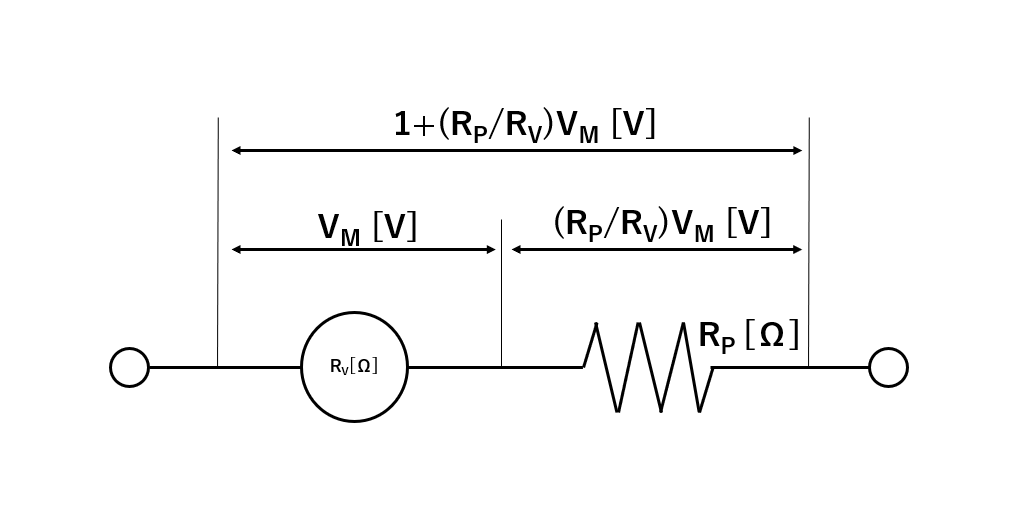
\includegraphics[width=10cm]{image/image01.png}
        \caption{測定範囲拡大時の各端子間抵抗}
    \end{center}
\end{figure}
これにより電圧計の最大目盛値$V_m$[V]は$(1+R_p/R_v)V_m$[V]まで拡張され\\
同値まで測定できる電圧計となる。測定値は指示値の$m$倍となり,$m$を倍率比という。\\
この時の最大目盛値を$V_{m_0}$と置くと,次式で表せる。

\begin{equation}
    V_{m_0}=(1+R_p/R_v)V_m
\end{equation}
\begin{equation}
    m=1+R_p/R_v
\end{equation}
\begin{equation}
    V_{m_0}=mV_m
\end{equation}

\section{実験内容}
\subsection{手順1 回路の作成}
\begin{figure}[H]
    \begin{center}
        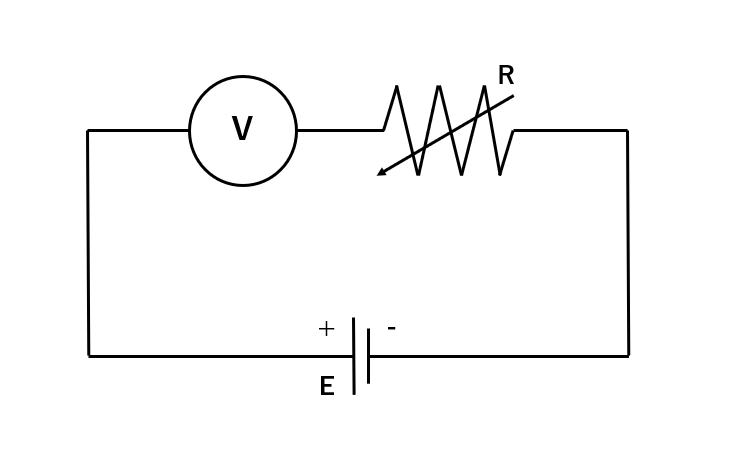
\includegraphics[width=8cm]{image/image02.png}
        \caption{測定範囲拡大法テスト回路}
    \end{center}
\end{figure}
図2のような回路を作成する。\\
E: 直流電源装置\\
V: 電圧器\\
R: 抵抗器
\subsection{手順2 倍率器抵抗値の決定}
電圧計Vの内部抵抗を10kΩとし,倍率比2,3倍とした時の抵抗値Rの値を求める。導出式は,
\begin{eqnarray}
    m &=& 1+R_p[Ω]/R_v[Ω] \nonumber\\
    m-1 &=& R_p[Ω]/R_v[Ω] \nonumber\\
    (m-1)*R_v[Ω] &=& R_p[Ω] \nonumber
\end{eqnarray}
これを実験回路の部品名に変更し,内部抵抗値及び倍率比を代入する。
\begin{eqnarray}
    (2-1)*10k[Ω] &=& R[Ω] \nonumber\\
    R[Ω] &=& 1*10k[Ω] \nonumber\\
    R[Ω] &=& 10k[Ω]
\end{eqnarray}
\begin{eqnarray}
    (3-1)*10k[Ω] &=& R[Ω] \nonumber\\
    R[Ω] &=& 2*10k[Ω] \nonumber\\
    R[Ω] &=& 20k[Ω]
\end{eqnarray}
式(4)より,倍率比2倍の場合は倍率器Rの抵抗値は10k[Ω]\\
式(5)より,倍率比3倍の場合は倍率器Rの抵抗値は20k[Ω]

\subsection{手順3 設定電圧を可変する}
直流電源装置Eの設定電圧を1[V]から10[V]まで1[V]毎に増加させる。\\
その都度、電圧計Vの指示値を読み記録する。
\subsection{手順4 指示値から測定値を計算}
電圧計Vの指示値と倍率比の積を求め測定値を決定,記録する。

\section{使用器具}
\begin{enumerate}
    \item 直流電源装置\\用途 直流電源確保のため\\商品名KIKUTU PMC18-3\\定格 INPUT AC100V 50/60Hz Max 230VA\\物品番号Ec-09
    \item 抵抗器\\用途 倍率器として使用するため\\商品名不明\\炭素皮膜抵抗器 10k[Ω]1本 20k[Ω]1本\\物品番号なし
    \item 電圧計\\用途 実験データ計測のため\\商品名YOKOGAWA MODEL2011 CLASS0.5 B9000EU\\定格 0-100V 1000Ω/V\\物品番号不明
\end{enumerate}

\section{実験結果}
\begin{table}[H]
    \centering
    \label{tab:tab`le1}
    \caption{計測結果【倍率器抵抗値10k[Ω]】}
    \begin{tabular}{c|c|c|c}
    設定電圧 E[V] & 電圧計V[V] & 倍率比m & 電圧Vm[V] \\
    \hline \hline
    1 & 0.5 & 2 & 1.0 \\\hline
    2 & 1.0 & 2 & 2.0 \\\hline
    3 & 1.5 & 2 & 3.0 \\\hline
    4 & 2.0 & 2 & 4.0 \\\hline
    5 & 2.5 & 2 & 5.0 \\\hline
    6 & 3.0 & 2 & 6.0 \\\hline
    7 & 3.5 & 2 & 7.0 \\\hline
    8 & 4.0 & 2 & 8.0 \\\hline
    9 & 4.5 & 2 & 9.0 \\\hline
    10 & 5.0 & 2 & 10.0 \\\hline
    \end{tabular}
\end{table}
\begin{table}[H]
    \centering
    \label{tab:tab`le2}
    \caption{計測結果倍率器抵抗値20k[Ω]】}
    \begin{tabular}{c|c|c|c}
    設定電圧 E[V] & 電圧計V[V] & 倍率比m & 電圧Vm[V] \\
    \hline \hline
    1 & 0.3 & 3 & 0.9 \\\hline
    2 & 0.7 & 3 & 2.1 \\\hline
    3 & 1.0 & 3 & 3.0 \\\hline
    4 & 1.3 & 3 & 3.9 \\\hline
    5 & 1.7 & 3 & 5.1 \\\hline
    6 & 2.0 & 3 & 6.0 \\\hline
    7 & 2.4 & 3 & 7.2 \\\hline
    8 & 2.7 & 3 & 8.1 \\\hline
    9 & 3.0 & 3 & 9.0 \\\hline
    10 & 3.4 & 3 & 10.2 \\
    \end{tabular}
\end{table}

\section{検証}
\begin{figure}[H]
    \begin{center}
        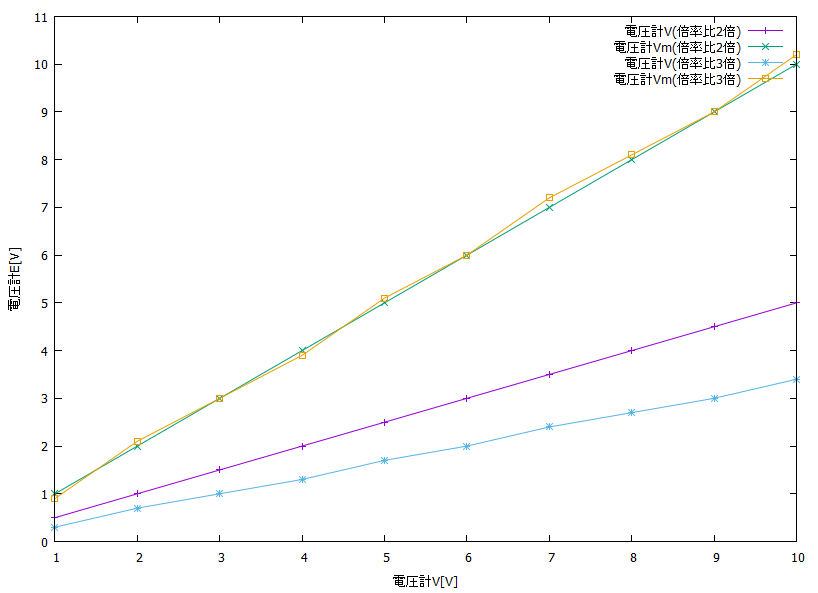
\includegraphics[width=10cm]{graph/graph01.png}
        \caption{電圧計の指示値V及び測定値Vmと設定電圧Eの関係}
    \end{center}
\end{figure}
倍率器によって測定範囲を拡張した計測において\\
電圧計の測定値Vmは,設定電圧Eと誤差±0.2[V]以下の精度で一致している。\\
また,指示値の傾きはそれぞれ測定値の傾きのほぼ$1/m$倍となっていおり,\\
これは倍率器によって倍率比に従った測定範囲拡張ができていることを示している。

\section{課題}
\subsection{(1)}
3V端子に18kΩの抵抗を直列接続して測定範囲を拡大すると,倍率比はいくらか。
\begin{eqnarray}
    倍率比をmとおく \nonumber\\
    3[V]*1000[Ω/V]=3000[Ω] \nonumber\\
    m=1+18k[Ω]/3000[Ω]=6 \nonumber\\
    m=7 \nonumber
    よって倍率比は7
\end{eqnarray}
\subsection{(2)}
(1)の状態で,針は2Vを示している。実際の電圧はいくらか。
\begin{eqnarray}
    7*2[V]=14[V] \nonumber\\
    よって14[V] \nonumber
\end{eqnarray}
\subsection{(3)}
10V端子に抵抗を直列接続し,電圧の測定範囲を拡大した。\\
30Vの直流電源を接続したところ,針は6Vを示した。抵抗の値はいくらか。
\begin{eqnarray}
    30[V]/6[v]=5 \nonumber\\
    倍率比は5倍 \nonumber\\
    10[V]*1000[Ω/V]=1000[Ω]=10k[Ω] \nonumber\\
    5-1*10k[Ω]=40000[Ω]=40k[Ω]\nonumber\\
    解は40k[Ω]\nonumber
\end{eqnarray}
\subsection{(4)}
24Vから72Vまで出力できる可変直流電源がある。これに電圧計を接続して調整作業を行いたい。\\
10V端子を使用するとして,倍率器抵抗はいくらが適当か。
\begin{eqnarray}
    可変直流電源の最大電圧72[V]を余裕をもって80[V]とする \nonumber\\
    80[V]/10[v]=8 \nonumber\\
    倍率比は8倍 \nonumber\\
    10[V]*1000[Ω/V]=1000[Ω]=10k[Ω] \nonumber\\
    8-1*10k[Ω]=70000[Ω]=70k[Ω]\nonumber\\
    よって70k[Ω]\nonumber\\
    しかし70k[Ω]の倍率器抵抗を接続しているということは電圧計の\nonumber\\
    測定値は1/7の解像度になっているということで,\nonumber\\
    今回のような調整作業では不向きな場合もあると考える\nonumber\\
    そのため必要に応じて倍率器抵抗を可変するべきだと考える。\nonumber\\
    24[V]/10[v]=2.4 \nonumber\\
    倍率比は2.4倍 \nonumber\\
    10[V]*1000[Ω/V]=1000[Ω]=10k[Ω] \nonumber\\
    2.4-1*10k[Ω]=14000[Ω]=14k[Ω]\nonumber\\
    よって14k[Ω]\nonumber\\
    倍率器抵抗は必要に応じて14k[Ω]から70k[Ω]の可変抵抗を用いるのが適当\nonumber
\end{eqnarray}

\end{document}